\section{Introduci\'on.}

\begin{frame}{Introducci\'on.}
	\begin{itemize}
		\item Se sabe que cada Aplicaci\'on tiene particularidades.
		\item Pero en general  siempre se repiten los mismos problemas:
			\begin{block}{Problemas recurrentes al desarrollar una aplicaci\'on}
			\begin{itemize}
				\item ?`C\'omo persisto los datos?
				\item ?`C\'omo autentifico a los usuarios?
				\item ?`C\'omo separo la presentaci\'on, la l\'ogica y control?.
			\end{itemize}
		\end{block}
					\item En lugar de reinventar continuamente una soluci\'on para cada nuevo proyecto. Es mucho mas
					productivo aplicar estrategias que ya hayan funcionado anteriormente.
					\item Esta idea es lo que lleva al concepto de \textit{ \textbf{Patr\'on de Diseño} }.
	\end{itemize}
\end{frame}

\begin{frame}{Patr\'on -> Un Modelo}
	\begin{itemize}
		\item En ingenier\'ia del software, un	patr\'on es una soluci\'on ya probada y aplicable a un
		problema que se presenta una y otra vez en el desarrollo de distintas aplicaciones y en
		distintos contextos.
		\item Un patr\'on no es una soluci\'on  codificada y lista para usar, sino más bien un \textbf{modelo}
		que describe c\'omo resolver el problema y de ante qu\'e circunstancias es aplicable.
		\item Si se decide aplicar un patr\'on, este debe ser previamente comunicado y documentado con el equipo del proyecto.
	\end{itemize}
\end{frame}

\begin{frame}{Patr\'on - Ventajas}
	\begin{itemize}
		\item \textbf{Están Probados:} son soluciones que han sido utilizadas con anterioridad de manera
		repetida y se ha comprobado que funcionan.
		\item \textbf{Son reutilizables:} corresponden con problemas que no son espec\'ificos de un caso
		concreto, sino que se presentan de forma recurrente en distintas aplicaciones.
		\item \textbf{Son expresivos:} cuando un equipo de desarrolladores tiene un vocabulario com\'un de
		patrones, se puede comunicar de manera fluida y precisa las ideas fundamentales sobre
		el dise\~no de una aplicaci\'on.
	\end{itemize}
\end{frame}

\begin{frame}{Patr\'on - Desventajas}
	\begin{itemize}
		\item Uso sin justificaci\'on que no aplica a un problema. (Simplemente porque son buenos)
		\item El an\'alisis y experiencia debe dictar si es necesario o no aplicarlos.
	\end{itemize}
\end{frame}


%\begin{frame}{Tips - Ocultamiento de Informaci\'on - Ejemplo.}
  %\begin{figure}
    %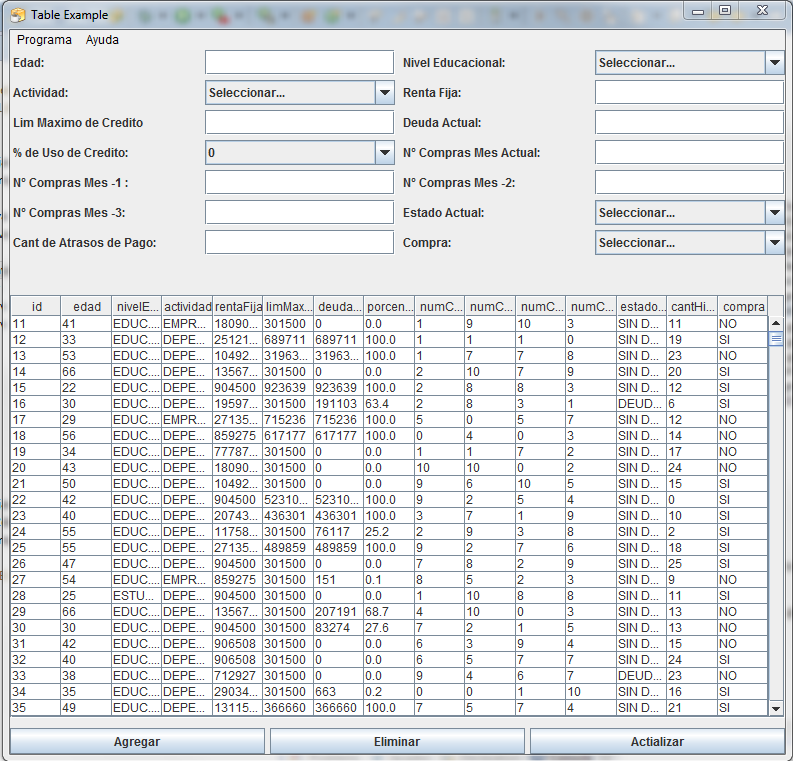
\includegraphics[scale=0.3]{figuras/DT.PNG}
  %\end{figure}
%\end{frame}

%\begin{frame}{Manejo de Excepciones - try, catch, finally}
%\begin{block}{Ejemplo.}
%\lstinputlisting[language=Java,caption={},numbers=none]{resources/excepciones/Finally.java}
%\end{block}
%\end{frame}
